\chapter{Lineær programmering}\label{Afsnit:LinProg}
Lineær programmering er en anvendelse af lineær algebra til at løse et optimeringsproblem. Lineære programmeringsproblemer tager udgangspunkt i maksimering eller minimering af en lineær funktion.
\begin{defn}[Lineær funktion]
Lad $f:\mathds{R} \to \mathds{R}$ være en funktion, da siges $f$ at være \textbf{lineær} hvis
\begin{enumerate}[label=\alph*]
\item $f(x_1 + x_2) = f(x_1) + f(x_2), \qquad \forall x_1,x_2 \in \mathds{R}$
\item $f(c\cdot x) = c \cdot f(x), \qquad \forall a, x \in \mathds{R}$
\end{enumerate}
\label{def:linfunk}
\end{defn}
Bemærk at selv om $f(x) = ax + b$ er kendt som en lineær funktion, er den ikke lineær pr Definition \ref{def:linfunk}.
Funktionen som skal optimeres kaldes objektfunktionen.
\begin{defn}
Betragt et lineært programmerings problem, da er \textbf{objektfunktionen}
\begin{align*}
f(\vec{x}) = \vec{c}^T \cdot \vec{x}, 
\end{align*}
for $\vec{x}, \vec{c} \in \mathds{R}^n$, funktionen, som ønskes optimeret.
\end{defn}
Objektfunktionen er repræsenteret som prikproduktet af en vektor $\vec{c}= \rvect{c_1 & c_2 & \cdots & c_n}^T$, der indeholder alle koefficienterne i funktionen og en vektor $\vec{x}= \rvect{x_1 & x_2 & \cdots & x_n}^T$, hvis indgange er funktionens variable.
Til objektfunktionen knyttes nogle bibetingelser, som variablene skal overholde. 
Eksistere der ingen bibetingelser, kan variablene tage en vilkårlig værdi, hvormed, hvis objektfunktionen skal minimeres, kan de variable med en negativ koefficient tage en vilkårlig højværdi, mens dem med positive koefficienter kan tage en vilkårlig høj negativ værdi, hvorfor løsningen vil blive $- \infty$.
\begin{defn}[bibetingelser]
Lad $\vec{x}\in \mathds{R}$ repræsentere variabelene til et lineært programmeringsproblem, og $x_i$ for den $i$ indgang i $\vec{x}$ da kaldes betingelser på formen
\begin{enumerate}
\item \textbf{positivitetsbetingelser}: $x_i \geq 0$
\item \textbf{lighedsbetingelser}: $\vec{a}_i^T\vec{x} = b_i$
\item \textbf{størreendbetingelser}: $\vec{a}_i^T\vec{x} \geq b_i$
\item \textbf{mindreendbetingelser}: $\vec{a}_i^T\vec{x} \leq b_i$
\end{enumerate}
for $\vec{a_i}\in \mathds{R}^n$ og $b_i\in \mathds{R}$. 
Er $x_i$ ikke betinget af en positivitetsbetingelse kaldes den for en \textbf{frivariable}.
\end{defn}
Her betegner vektoren $\vec{a_i}$ koefficienterne i den $i$ bibetingelse, bemærk at hvis en ligning ikke indeholder den $j$ variable, da vil den $j$te indgang i koefficientvektoren $\vec{a_i}$ være lig nul, da der skal være en indgang pr variabel, ellers er prikproduktet ikke defineret. 
Da bibetingelserne er ligninger repræsenteret ved et prikprodukt, kan hele ligningssystemet repræsenteres som et matrix-vektorprodukt, det kræver dog, at alle ikke positivitets betingelser er på samme form.
Det kan derfor være favorabelt at kunne omskrive fra en ulighed til en anden.
\begin{stn}
Lad $\vec{a}_i^T,\vec{x} \in \mathds{R}^n$ og $b_i \in \mathds{R}$, da gælder:
\begin{enumerate}
\item $\vec{a}_i^T\vec{x} \geq b_i \quad \Leftrightarrow \quad -\vec{a}_i^T\vec{x} \leq -b_i$
\item $\vec{a}_i^T\vec{x} = b_i \quad \Leftrightarrow  \quad  \vec{a}_i^T\vec{x} \leq b_i \quad \wedge \quad  \vec{a}_i^T\vec{x} \geq b_i$
\item $\vec{a}_i^T \vec{x}  \leq b_i \quad \Rightarrow \quad  \vec{a}_i^T \vec{x}  +  x_{n+i}  = b_i$
\item $\vec{a}_i^T \vec{x}  \geq b_i \quad \Rightarrow \quad  \vec{a}_i^T \vec{x}  - x_{n+i}  = b_i$
\end{enumerate}
hvor $x_{n+i}$ er en slack variable. 
\end{stn}
Dermed kan bibetingelserne skrives som $A\vec{x}\geq \vec{b}$, hvor $\vec{a_i}$ udgør den $i$te række i $A$ og $b_i$ er den $i$ indgang i $\vec{b}$.
Bemærk at positivitetsbetingelserne er et særtilfælde af størreendbetingelser, hvor en koefficienten til $x_i$ er 1, mens resten af koefficienterne er 0 og hvor $b_i=0$.
Positivitets betingelsen skrives ikke med i ligningssystemet, og i stedet er det som oftes underforstået, at enhver variable skal være ikke negativ.
For at det skal gøre sig gældende, skal en hver frivariable omskrives så de er betinget af en positivitetsbetingelse.
\begin{stn}
Lad $x_i$ være en frivariabel, da er $x_i = x_{n+i}-x_{n+i+1}$, hvor $x_{n+i},x_{n+i+1}\geq 0$.
\end{stn}
Det betyder at et hvert lineært programmerings problem kan omskrives så det står på standardform.
\begin{defn}[Standard minimumsproblemer]
Lad $f(\vec{x}) = \vec{c}^T\vec{x}$ betegne objektfunktionen til et lineært minimeringsproblem, for $\vec{x},\vec{c} \in\mathds{R}^n$, lad $m \times n$ matricen $A=[A_{ij}]$ for $i=1,...,m$ og $j=1,...,n$, og lad $\vec{b} \in  \mathds{R}^n$.
Der er standard minimumsproblemet defineret som\\
\begin{center}
\begin{tabular}{l	>{$}l<{$}}
Minimer			& \vec{c}^T\vec{x} \\
med hensyn til 	& A\vec{x} \geq \vec{b}\\
og 				& \vec{x} \geq \vec{0}.
\end{tabular}
\end{center}
Består ligningssystemet af ligheder kaldes problemet; \textbf{standard minimumsproblem med ligheder}.
\label{def:std_maksmin}
\end{defn}
Bemærk at på samme måde som bibetingelserne kan omskrives, kan et minimeringsproblem laves til et maksimeringsproblem ved at multiplicere med $-1$, hvorfor at alle definitioner og sætninger er ækvivalente. Derfor defineres begreber og sætninger kun for minimums problemer, mens eksemplerne illustrere maksimums problemer.
\begin{eks}[Standard maksimumsproblem]
Hvis eksempel \ref{eks:maksprob1} skal omskrives til et standard maksimumsproblem, skal alle relationer i bibetingelserne være mindre end eller lig med.
Bibetingelse nr. 3 skal derved omskrives. Dette kan gøres ved at multiplicere begge sider af uligheden med $-1$, da dette vender ulighedstegnet. Derved bliver Eksempel \ref{eks:maksprob1} omskrevet til et standard maksimumsproblem.\\
\begin{center}
\begin{tabular}{l	>{$}r<{$}	>{$}r<{$}	>{$}l<{$}}
Maksimer 		& 		4x_1	&	+3 x_2	& \\
med hensyn til 	&  \ \ 	-2 x_1	& 	+4 x_2	& \leq 8\\
				&  		x_1		& 	+3 x_2	& \leq 16\\
				&  \ \ 	x_1		& 			& \leq 10\\
og $x_1 \geq 0, x_2\geq 0$.
\end{tabular}
\end{center}
\label{eks:maksprob2}
\end{eks}

\section{Løsninger til linære programmeringsproblemer}
Den mulige mængde er mængden af løsningsvektorer, $\vec{x}$, som opfylder alle problemets betingelser. Hvis en optimal løsning eksisterer vil denne derved være indeholdt i den mulige mængde.
\begin{defn}[Mulige løsninger og den mulige mængde]
Lad $A\vec{x}\geq \vec{b}$ betegne et lineært programmerings problem på standard form. 
Da er $\vec{x^*}$ n \textbf{mulig løsning} hvis og kun hvis $A \vec{x^*} \geq \vec{b}$ og $\vec{x^*}\geq \vec{0}$.\\
\textbf{Den mulige mængde} er mængden
\begin{align*}
\mathcal{F}=\{\vec{x} \in \mathds{R}^n|A\vec{x} \geq \vec{b}, \vec{x} \geq \vec{0}\}
\end{align*}
Et problem kaldes \textbf{inkonsistent}, hvis den mulige mængde er den tomme mængde, ellers er problemet \textbf{konsistent}.
\end{defn}
I lineære programmering ledes der efter en optimal løsning, som vil være den mulige løsning, der enten maksimere objektfunktionen eller minimere den, alt afhængig af om der er tale om et minimeringsproblem. 
Bemærk at på samme måde som bibetingelserne kan omskrives, kan et minimeringsproblem laves til et maksimeringsproblem ved at multiplicere med $-1$, hvorfor det kun er nødvendigt at definere den optimale løsning for minimeringsproblemet.
\begin{defn}[Optimal løsning]
Lad $f$ være objektfunktionen til et lineært minimeringsproblem, da kaldes en vektor $\vec{x}^*$ en \textbf{optimal løsning}, hvis 
\begin{align}
	f(\vec{x}^*)=\min\limits_{\vec{x} \in \mathcal{F}}f(\vec{x}).
\end{align}
Værdien af $f(\vec{x^*})$ kaldes den \textbf{optimale værdi}.
\end{defn}

Den optimale løsning kan findes på forskellige måder heriblandt med simplex-metoden, som beskrives i Kapitel \ref{afsnit:simplex}. En anden måde er ved geometrisk visualisering af den mulige mængde. Denne metode er mulig for problemer med op til 3 variable, da løsningsmængden derved visualiseres som et plot i det tilsvarende antal dimensioner. 

\begin{eks}[Den mulige mængde]
Ved at indtegne betingelserne i et koordinatsystem, er det muligt at visualisere den mulige mængde som fællesmængden af de mængder, der dannes ud fra betingelserne. På Figur \ref{fig:maksprob2} er den mulige mængde for problemet i Eksempel \ref{eks:maksprob2} indtegnet. Der er desuden tegnet en pil for hver betingelse, som viser for hvilken side af linjen, at koordinaterne opfylder betingelsen. Den mulige mængde er farvet grå.

\begin{center}
	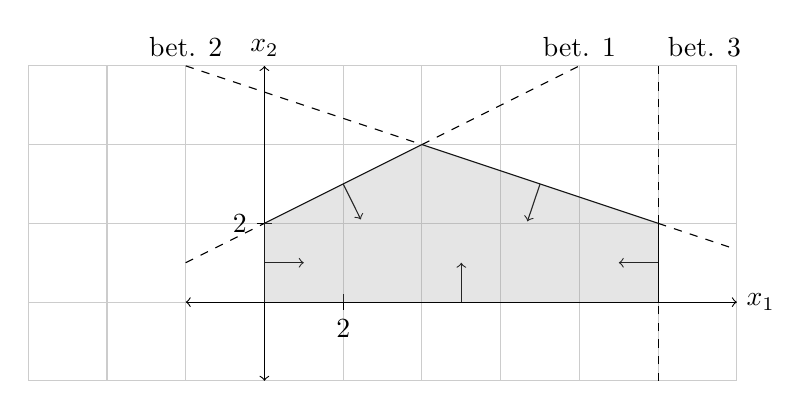
\begin{tikzpicture}
  %laver Grid. godt til når koordinater skal redigeres
  	\draw[thin,gray!40] (-3,-1) grid (6,3); 
  %x-aksen
  	\draw[<->] (-1,0)--(6,0) node[right]{$x_1$};
  	\draw[->] (2.5,0) -- (2.5,0.5);
  %y-aksen
  	\draw[<->] (0,-1)--(0,3) node[above]{$x_2$};
  	\draw[->] (0,0.5) -- (0.5,0.5);
  	
  %akse-markeringer
  	%\node[left] (xakse) at (0,1) {2};
  	\draw[] (-0.1,1) -- (0.1,1) node[pos=0,left] {2};
  	\draw[] (1,-0.1) -- (1,0.1) node[pos=0,below] {2};
  	
  %ligning 1
	\draw[domain=-1:0,variable=\x,dashed] 	plot({\x},{0.5*\x+1});
	\draw[domain=0:2,variable=\x] 			plot({\x},{0.5*\x+1});
	\draw[domain=2:4,variable=\x,dashed] 	plot({\x},{0.5*\x+1}) node[above] {bet. 1};
  	\draw[->] (1,1.5) -- (1.224,1.05);
	
  %ligning 2
  	\draw[domain=-1:2,variable=\x,dashed] 	plot({\x},{-(1/3)*\x+8/3}) node[above] at (-1,3) {bet. 2} ;
	\draw[domain=2:5,variable=\x] 			plot({\x},{-(1/3)*\x+8/3});
	\draw[domain=5:6,variable=\x,dashed] 	plot({\x},{-(1/3)*\x+8/3});
	\draw[->] (3.5,1.5) -- (3.34,1.026);

  %ligning 3
  	\draw[domain=-1:0,variable=\y,dashed] 	plot({5},{\y});
	\draw[domain=0:1,variable=\y] 			plot({5},{\y});
	\draw[domain=1:3,variable=\y,dashed] 	plot({5},{\y}) node[above right] {bet. 3};
	\draw[->] (5,0.5) -- (4.5,0.5);

  %løsningsmængden skraveret
	\fill[gray!80,nearly transparent] (0,0) -- (0,1) -- (2,2) -- (5,1) --(5,0) --  cycle;
\end{tikzpicture}
	\captionof{figure}{Skravering af den mulige mængde for et standard maksimeringsporblem.}
	\label{fig:maksprob2}
\end{center}

\end{eks}

\subsection{Niveaukurver}
En måde at finde den optimale løsning for lineære programmerings problemer med få variable er ved introduktionen af niveaukurver.
\begin{defn}[Niveaukurver]
Lad $f(\vec{x})= \vec{c}^T\vec{x}$ være en funktion, da er en \textbf{niveaukurve} mængden 
\begin{align*}
N_z = \{\vec{x}| f(\vec{x}) = z, z \in \mathds{R}\}
\end{align*}
\end{defn}
Niveau kurver er dermed den mængde af vektorer, der har samme funktionsværdi for objektfunktionen. 
De vektorer udspænder en linje, som er ortogonal med koefficentvektoren $\vec{c}$.
\begin{stn}[Niveaukurven er ortogonal med $\vec{c}$]
Lad $N_z$ betegne en niveaukurve, til objektfunktionen $f(\vec{x})= \vec{c}^T\vec{x}$, da er $\vec{c}$ ortogonal med linjen udspændt af $N_z$.
\end{stn}
\begin{proof}
Lad $\vec{x}, \vec{y} \in N_z$ da er linjen udspændt af $N_z$ parallel med differensvektoren $\vec{x}-\vec{y}$.
Tages prikproduktet af differensvektoren og vektor $\vec{c}$, fåes at
\begin{align*}
\vec{c}^T(\vec{x}-\vec{y}) = \vec{c}^T\vec{x} -\vec{c}^T\vec{y} = z - z = 0,
\end{align*}
hvorfor at vektor $\vec{c}$ og differencevektoren er ortogonale, og dermed må vektor $\vec{c}$ også være orthogonal med linjen udspændt af $N_z$.
\end{proof}
Den optimale løsning findes så ved at finde det mindste $z$ for hvilken niveaukurven har en ikke-tom skæring med den mulige mængde. 
Hvilket gøres ved at flytte kurven så langt i den modsatte retningen af $\vec{c}$ som muligt.
\begin{stn}[Optimal løsning og -værdi fundet ved niveaukurver]
Lad $f(\vec{x})=\vec{c}^T\vec{x}$ betegne objektfunktionen til et standard minimerings problem med løsningsmængde $\mathcal{F}$, da vil den optimale løsning være givet ved 
\begin{align*}
\vec{x^*}=\underset{k}{\min} \, k \cdot \vec{c} \in \mathcal{F}.
\end{align*}
og den optimale værdi er givet ved
\begin{align*}
z^* = \underset{k}{\min} \, k \cdot \Vert \vec{c} \Vert ^2
\end{align*}
\label{stn:niveau}
\end{stn}
\begin{proof}
Det følger af Sætning %mangler
, at en løsningsvektor $\vec{x}$ kan omskrives til summen af en vektor parallel med $\vec{c}$, kaldet $\vec{x}_p$, og en vektor orthogonal med $\vec{c}$, kaldet $\vec{x}_o$. 
Dermed kan objektfunktionen omskrives til
\begin{align*}
	f(\vec{x}) & \ = \ \vec{c}^T\vec{x}\\
	f(\vec{x_p}+\vec{x_o}) & \ = \ 
	\vec{c}^T\vec{x_p}+\vec{c}^T\vec{x_o} \ = \ 
	\vec{c}^T\vec{x_p} \ = \ 
	k\cdot \vec{c}^T\vec{c} \ = \ 
	k \cdot \Vert \vec{c} \Vert ^2.
\end{align*}
Dermed kan det konkluderes at den optimale løsning er en vektor $\vec{x^*}=\underset{k}{min} k \cdot \vec{c} \in \mathcal{F}$, og den optimale værdi er $z* = \underset{k}{min}k \cdot \Vert \vec{c} \Vert ^2$
\end{proof}
Af Sætning \ref{stn:niveau} følger det også, at den optimale værdi er den vinkelrette afstand fra origo og  linjen udspændt af niveaukurven. 
Det følger af at den optimale værdi er givet, som et multiplum af længden af $\vec{c}$, der står vinkelret på linjen udspændt af niveaukurven.
i
Dette kan ses i  for et maksimerings problem i Eksempel \ref{eks:maksprob3}.


\begin{eks}[Optimal løsning fundet grafisk]
Niveaukurverne $46=\vec{c}^T \vec{x}$ og $25=\vec{c}^T \vec{x}$ er på Figur \ref{fig:maksprob3} indtegnet for programmeringsprogblemet fra Eksempel \ref{eks:maksprob2}.

	\begin{center}	
		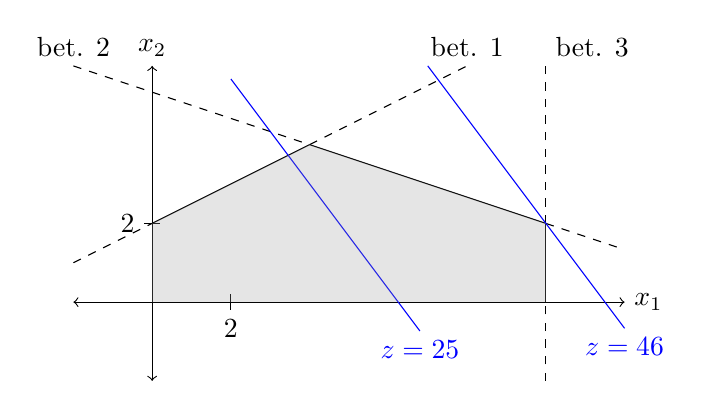
\begin{tikzpicture}
  %laver Grid. godt til når koordinater skal redigeres
  	%\draw[thin,gray!40] (-3,-1) grid (6,3); 
  %x-aksen
  	\draw[<->] (-1,0)--(6,0) node[right]{$x_1$}; 
  %y-aksen
  	\draw[<->] (0,-1)--(0,3) node[above]{$x_2$};
  	
  %akse-markeringer
  	%\node[left] (xakse) at (0,1) {2};
  	\draw[] (-0.1,1) -- (0.1,1) node[pos=0,left] {2};
  	\draw[] (1,-0.1) -- (1,0.1) node[pos=0,below] {2};
  	
  %ligning 1
	\draw[domain=-1:0,variable=\x,dashed] 	plot({\x},{0.5*\x+1});
	\draw[domain=0:2,variable=\x] 			plot({\x},{0.5*\x+1});
	\draw[domain=2:4,variable=\x,dashed] 	plot({\x},{0.5*\x+1}) node[above] {bet. 1};
	
  %ligning 2
  	\draw[domain=-1:2,variable=\x,dashed] 	plot({\x},{-(1/3)*\x+8/3}) node[above] at (-1,3) {bet. 2} ;
	\draw[domain=2:5,variable=\x] 			plot({\x},{-(1/3)*\x+8/3});
	\draw[domain=5:6,variable=\x,dashed] 	plot({\x},{-(1/3)*\x+8/3});
	

  %ligning 3
  	\draw[domain=-1:0,variable=\y,dashed] 	plot({5},{\y});
	\draw[domain=0:1,variable=\y] 			plot({5},{\y});
	\draw[domain=1:3,variable=\y,dashed] 	plot({5},{\y}) node[above right] {bet. 3};
	
  %niveaukurver
  	\draw[domain=3.5:6,variable=\x,blue] plot({\x},{-(4/3)*\x+23/3}) node[below] {$z=46$};
  	\draw[domain=1:3.4,variable=\x,blue] plot({\x},{-(4/3)*\x+25/6}) node[below] {$z=25$};
  	
  %c-vektor
  	%\draw[->,thick,red] (0,0) -- (2,1.5);

  %løsningsmængden skraveret
	\fill[gray!80,nearly transparent] (0,0) -- (0,1) -- (2,2) -- (5,1) --(5,0) --  cycle;
\end{tikzpicture}
		\captionof{figure}{Optimal løsning i den mulige mængde fundet som skæring med ligningen $z=46$.}
		\label{fig:maksprob3}
	\end{center}
	
På figuren ses det, at den største funktionsværdi $z=46$ findes i skæringen mellem bibetingelse 2 og 3.
Ved at løse bibetingelse 2 og 3 som 2 ligninger med 2 ubekendte findes det at den optimale løsning er $\vec{x}=\rvect{10 & 2}^T.$
\label{eks:maksprob3}
\end{eks}


